\chapter{Introduction}
\label{chap: Introduction}


\section{Background and Motivation}
Turbulent flows are found in a wide range of natural and engineering systems, from large-scale atmospheric flows and ocean currents to industrial processes and aerodynamic applications. Over the past decades, Computational Fluid Dynamics (CFD) has proven itself to be an effective and powerful means of simulating unsteady fluid flow, both laminar and turbulent. It has proven its use across various industries, where it has played a central role in the analysis, design, and certification of aerospace vehicles, environmental systems, industrial products, and even healthcare developments. Advances in numerical methods and high-performance computing (HPC) have ensured steady advances in reliability and accuracy of CFD, making it a critical element in modern engineering workflows \cite{Spalart2016}. 

\subsection{Need for high-fidelity yet efficient simulation}

% \begin{wrapfigure}{r}{0.5\textwidth}
% \vspace{-1.5em}
%      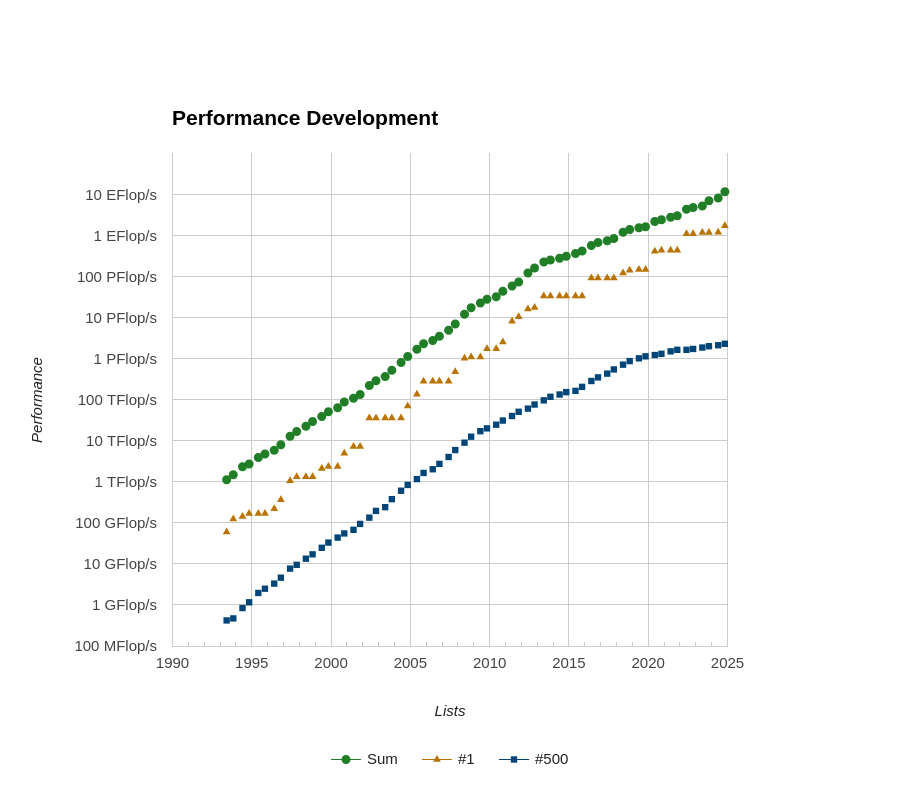
\includegraphics[width=\linewidth]{figures/Moore.png}
%     \caption{Performance trends of the TOP500 supercomputers (1993–2025), showing total performance (Sum), top system ($\#$1), and 500th system ($\#$500). Performance is in FLOP/s on a logarithmic scale. Adapted from \textcite{top500}}
%     \label{fig: Moore}
% \end{wrapfigure}

\begin{figure}
    \centering
    % 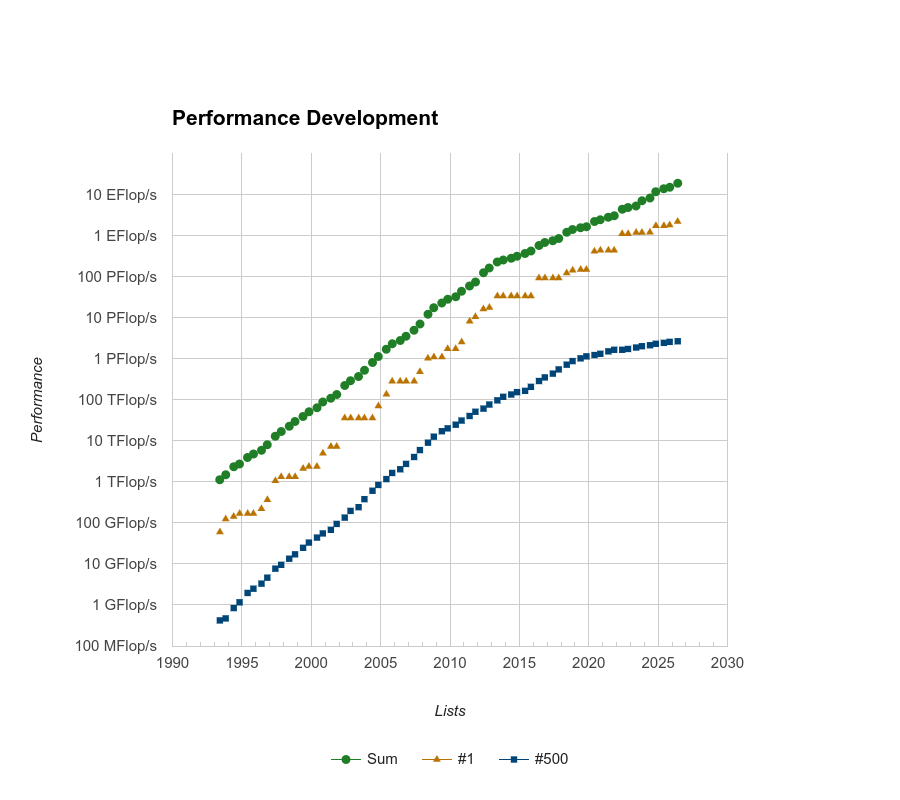
\includegraphics[width=.85\linewidth]{figures/Literature review/TOP500.png}
    % ====================================================================
% TOP500 Performance Development figure  --  drop-in TikZ/pgfplots block
% Preamble of your document must contain:
%   \usepackage{pgfplots}
%   \pgfplotsset{compat=1.18}
% (and optionally \usepackage{helvet} for the sans-serif look)
% ====================================================================

% ----- colors -----
\definecolor{sumgreen}{RGB}{46,139,46}
\definecolor{onegold}{RGB}{210,140,20}
\definecolor{fiveblue}{RGB}{15,60,130}
\definecolor{gridgray}{RGB}{210,210,210}
\definecolor{bordergray}{RGB}{120,120,120}

% ----- data (year, FLOP/s) -----
\def\sumcoords{(1993.4,1.1e+12) (1993.9,1.41686e+12) (1994.4,1.82499e+12) (1994.9,2.35069e+12) (1995.4,3.02782e+12) (1995.9,3.9e+12) (1996.4,4.89769e+12) (1996.9,6.15061e+12) (1997.4,7.72405e+12) (1997.9,9.7e+12) (1998.4,1.26435e+13) (1998.9,1.64803e+13) (1999.4,2.14813e+13) (1999.9,2.8e+13) (2000.4,3.72811e+13) (2000.9,4.96387e+13) (2001.4,6.60924e+13) (2001.9,8.8e+13) (2002.4,1.53421e+14) (2002.9,2.67477e+14) (2003.4,4.66325e+14) (2003.9,8.13e+14) (2004.4,1.05439e+15) (2004.9,1.36744e+15) (2005.4,1.77345e+15) (2005.9,2.3e+15) (2006.4,3.03462e+15) (2006.9,4.00387e+15) (2007.4,5.28271e+15) (2007.9,6.97e+15) (2008.4,1.08693e+16) (2008.9,1.695e+16) (2009.4,2.17464e+16) (2009.9,2.79e+16) (2010.4,3.49055e+16) (2010.9,4.367e+16) (2011.4,5.69238e+16) (2011.9,7.42e+16) (2012.4,9.56885e+16) (2012.9,1.234e+17) (2013.4,1.75747e+17) (2013.9,2.503e+17) (2014.4,2.78106e+17) (2014.9,3.09e+17) (2015.4,3.6025e+17) (2015.9,4.2e+17) (2016.4,4.87867e+17) (2016.9,5.667e+17) (2017.4,6.91998e+17) (2017.9,8.45e+17) (2018.4,1.09463e+18) (2018.9,1.418e+18) (2019.4,1.52961e+18) (2019.9,1.65e+18) (2020.4,2.00237e+18) (2020.9,2.43e+18) (2021.4,2.71794e+18) (2021.9,3.04e+18) (2022.4,3.84375e+18) (2022.9,4.86e+18) (2023.4,5.83267e+18) (2023.9,7e+18) (2024.4,9.05759e+18) (2024.9,1.172e+19) (2025.4,1.23434e+19) (2025.9,1.3e+19)}
\def\onecoords{(1993.4,5.97e+10) (1993.9,1.24e+11) (1994.4,1.43e+11) (1994.9,1.7e+11) (1995.4,1.7e+11) (1995.9,1.7e+11) (1996.4,2.2e+11) (1996.9,3.68e+11) (1997.4,1.068e+12) (1997.9,1.068e+12) (1998.4,1.338e+12) (1998.9,1.338e+12) (1999.4,2.121e+12) (1999.9,2.379e+12) (2000.4,2.379e+12) (2000.9,4.938e+12) (2001.4,7.226e+12) (2001.9,7.226e+12) (2002.4,3.586e+13) (2002.9,3.586e+13) (2003.4,3.586e+13) (2003.9,3.586e+13) (2004.4,3.586e+13) (2004.9,7.072e+13) (2005.4,1.368e+14) (2005.9,2.806e+14) (2006.4,2.806e+14) (2006.9,2.806e+14) (2007.4,2.806e+14) (2007.9,4.782e+14) (2008.4,1.105e+15) (2008.9,1.105e+15) (2009.4,1.105e+15) (2009.9,1.759e+15) (2010.4,1.759e+15) (2010.9,2.566e+15) (2011.4,8.162e+15) (2011.9,1.051e+16) (2012.4,1.632e+16) (2012.9,1.759e+16) (2013.4,3.3862e+16) (2013.9,3.3862e+16) (2014.4,3.3862e+16) (2014.9,3.3862e+16) (2015.4,3.3862e+16) (2015.9,3.3862e+16) (2016.4,9.3014e+16) (2016.9,9.3014e+16) (2017.4,9.3014e+16) (2017.9,9.3014e+16) (2018.4,1.223e+17) (2018.9,1.435e+17) (2019.4,1.486e+17) (2019.9,1.486e+17) (2020.4,4.1553e+17) (2020.9,4.4201e+17) (2021.4,4.4201e+17) (2021.9,4.4201e+17) (2022.4,1.102e+18) (2022.9,1.102e+18) (2023.4,1.194e+18) (2023.9,1.194e+18) (2024.4,1.206e+18) (2024.9,1.742e+18) (2025.4,1.742e+18) (2025.9,1.742e+18)}
\def\fivehcoords{(1993.4,4e+08) (1993.9,4.82028e+08) (1994.4,5.80879e+08) (1994.9,7e+08) (1995.4,9.16515e+08) (1995.9,1.2e+09) (1996.4,1.48312e+09) (1996.9,1.83303e+09) (1997.4,2.2655e+09) (1997.9,2.8e+09) (1998.4,3.44281e+09) (1998.9,4.2332e+09) (1999.4,5.20504e+09) (1999.9,6.4e+09) (2000.4,8.9061e+09) (2000.9,1.23935e+10) (2001.4,1.72466e+10) (2001.9,2.4e+10) (2002.4,4.8583e+10) (2002.9,9.83463e+10) (2003.4,1.99082e+11) (2003.9,4.03e+11) (2004.4,5.7291e+11) (2004.9,8.14456e+11) (2005.4,1.15784e+12) (2005.9,1.646e+12) (2006.4,2.26483e+12) (2006.9,3.11631e+12) (2007.4,4.28792e+12) (2007.9,5.9e+12) (2008.4,8.63574e+12) (2008.9,1.264e+13) (2009.4,1.59195e+13) (2009.9,2.005e+13) (2010.4,2.49711e+13) (2010.9,3.11e+13) (2011.4,3.97868e+13) (2011.9,5.09e+13) (2012.4,6.24007e+13) (2012.9,7.65e+13) (2013.4,9.493e+13) (2013.9,1.178e+14) (2014.4,1.34514e+14) (2014.9,1.536e+14) (2015.4,1.7801e+14) (2015.9,2.063e+14) (2016.4,2.68441e+14) (2016.9,3.493e+14) (2017.4,4.37791e+14) (2017.9,5.487e+14) (2018.4,6.92822e+14) (2018.9,8.748e+14) (2019.4,9.99511e+14) (2019.9,1.142e+15) (2020.4,1.22638e+15) (2020.9,1.317e+15) (2021.4,1.47368e+15) (2021.9,1.649e+15) (2022.4,1.68901e+15) (2022.9,1.73e+15) (2023.4,1.92321e+15) (2023.9,2.138e+15) (2024.4,2.26993e+15) (2024.9,2.41e+15) (2025.4,2.48387e+15) (2025.9,2.56e+15)}

% ----- figure -----
\
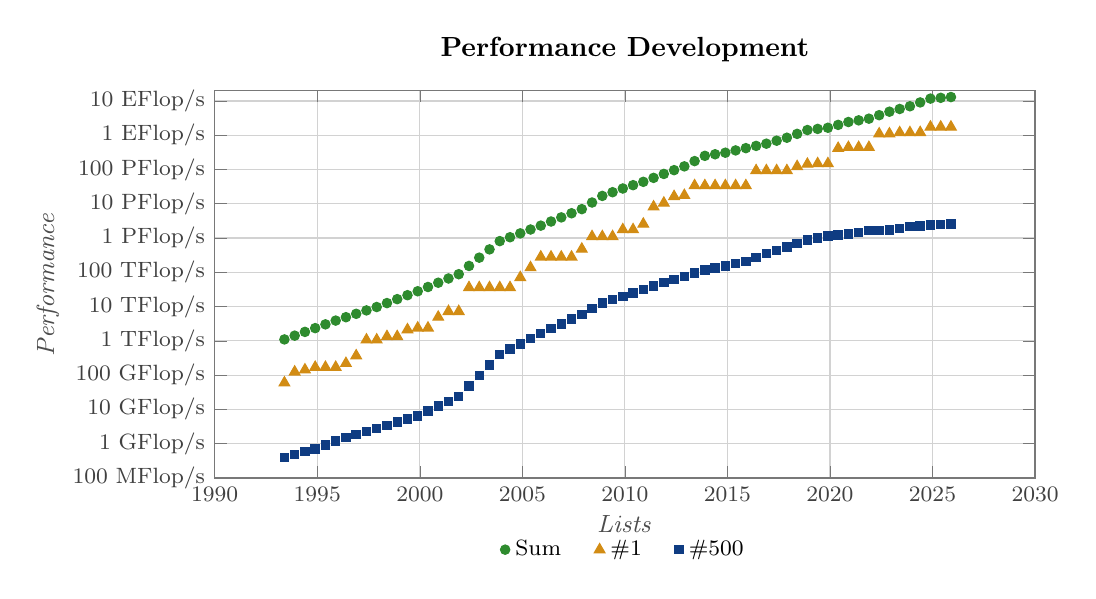
\begin{tikzpicture}
\begin{axis}[
    width=12cm, height=6.5cm,
    title=\textbf{Performance Development},
    title style={font=\bfseries, yshift=1pt},
    ymode=log, log basis y=10,
    xmin=1990, xmax=2030,
    ymin=1e8, ymax=2e19,
    xtick={1990,1995,2000,2005,2010,2015,2020,2025,2030},
    ytick={1e8,1e9,1e10,1e11,1e12,1e13,1e14,1e15,1e16,1e17,1e18,1e19},
    yticklabels={100 MFlop/s,1 GFlop/s,10 GFlop/s,100 GFlop/s,%
        1 TFlop/s,10 TFlop/s,100 TFlop/s,1 PFlop/s,10 PFlop/s,%
        100 PFlop/s,1 EFlop/s,10 EFlop/s},
    tick label style={font=\footnotesize, color=black!75},
    scaled x ticks=false,
    xticklabel style={/pgf/number format/1000 sep={}},
    reverse legend,
    xlabel={\textit{Lists}}, ylabel={\textit{Performance}},
    label style={font=\small, color=black!70},
    xlabel style={yshift=2pt}, ylabel style={yshift=-2pt},
    grid=both,
    major grid style={color=gridgray, line width=0.4pt},
    minor tick num=0,
    axis line style={color=bordergray, line width=0.5pt},
    tick style={color=bordergray},
    enlargelimits=false,
    legend style={
        at={(0.5,-0.13)}, anchor=north, legend columns=3,
        draw=none, fill=none, font=\footnotesize,
        /tikz/every even column/.append style={column sep=10pt}},
    legend image post style={mark options={scale=1}},
    clip mode=individual,
]

% #500 (blue squares)
\addplot[fiveblue, only marks, mark=square*, mark size=1.5pt,
    mark options={fill=fiveblue, draw=fiveblue}] coordinates {\fivehcoords};
\addlegendentry{\#500}

% #1 (gold triangles)
\addplot[onegold, only marks, mark=triangle*, mark size=2.2pt,
    mark options={fill=onegold, draw=onegold}] coordinates {\onecoords};
\addlegendentry{\#1}

% Sum (green circles)
\addplot[sumgreen, only marks, mark=*, mark size=1.7pt,
    mark options={fill=sumgreen, draw=sumgreen}] coordinates {\sumcoords};
\addlegendentry{Sum}

\end{axis}
\end{tikzpicture}
    \caption{Performance trends of the TOP500 supercomputers (1993–2026), showing total performance (Sum), top system ($\#$1), and 500th system ($\#$500). Performance is in FLOP/s on a logarithmic scale. Adapted from \textcite{top500}}
    \label{fig: Moore}
\end{figure}

Even with the technological advancements of the last few decades, the computational cost of accurate CFD simulations remains a bottleneck. This is especially the case if one aims to resolve unsteady, turbulent flows in or around complex geometries. These types of simulations require a mesh of such high quality that even the smallest and most complex flow phenomena can be captured accurately \cite{Spalart2000}. This presents two problems, each of which requires substantial time to evaluate: one is fabricating the mesh through which we want to apply our CFD algorithms, and the other is considering the CFD algorithms and the subsequent turbulence models. In practice, companies navigate a spectrum of methods that trade computational efficiency for accuracy, ranging from Reynolds Averaged Navier–Stokes (RANS) to Large-Eddy Simulation (LES), hybrid RANS–LES approaches, and ultimately Direct Numerical Simulation (DNS) to gain a competitive edge in the highly competitive aeronautical markets \cite{Spalart2000}. This indicates the need for frameworks that can decrease the computational costs of high-fidelity CFD simulations. 

Compounding this is the slowing of hardware-driven performance gains. Ever since 1965, following Gordon Moore's observation \cite{moore1965}, the number of transistors in a single integrated circuit has doubled approximately every two years, while cost, power, and area have remained fixed. However, as transistors reach the atomic scale and fabrication costs continue to rise, the classical technological driver underpinning Moore's Law for 50 years is failing and is anticipated to have flattened by 2025 \cite{Shalf2020}, as shown in \autoref{fig: Moore}. This 'death march' of Moore's Law \cite{Markov2014} opens the door for new hard- and software architectures, as well as creative CFD workflows. 

Besides the recent flattening of Moore's Law, researchers have been passionately innovating for several decades and finding novel ways to reduce the computational cost of CFD simulations. One way to accelerate CFD simulations is to employ advances in multicore computer architecture developed over the last few decades \cite{Hosain2015}. These novel methods enable the use of multicore and manycore CPU (Central Processing Unit) architectures \cite{Hadade2016}, as well as GPUs (Graphics Processing Units) to accelerate CFD solvers \cite{Xiang2017}. To achieve desirable acceleration results, these hardware methods have been paired with advanced numerical schemes that employ mesh-based, mesh-free, or hybrid methods to achieve significant simulation speed-ups \cite{Hosain2015}. 

Together with advances in computing architecture, the rapid progress in Machine Learning (ML) and Artificial Intelligence (AI) offers promising new strategies for accelerating CFD simulations. Fluid mechanics has always been a field where an enormous amount of data must be handled. This can be derived from either experimental results or large-scale numerical simulations \cite{Brunton2020}. Together with these vast amounts of data and the ability to handle them, ML offers a promising outlook for accelerating modern unsteady CFD simulations.

It is in this landscape that the subject of this thesis finds itself. Bounded by the computational bottleneck created by accurate CFD simulations, and driven by technological advancements in AI technology. This thesis aims to develop a new approach to reducing the computational costs of unsteady flow simulations by leveraging modern AI frameworks. More specifically, this work will focus on using neural ordinary differential equations to accelerate the time integration step. Since this is, more often than not, the most costly part in mesh-based solving algorithms. In light of this context, this thesis aims to answer the following central research question and subquestions:


\begin{center}
\begin{minipage}{\textwidth}
\begin{tcolorbox}[colback=gray!5,colframe=black!80,title=Research Question]
\textbf{How effectively can neural ordinary differential equations accelerate the time integration step in CFD solvers for unsteady simulations without compromising accuracy?}
\vspace{1em}

\begin{enumerate}
  % \item To what extent can neural ODE architectures maintain physical accuracy across different unsteady flow regimes, Reynolds numbers, and geometric configurations (e.g., symmetric, asymmetric, irregular shapes)?
    % \vfill
    \item How well does the neural ODE acceleration framework preserve the flow's statistical observables when transferred across Reynolds numbers and grid resolution?
    \vspace{0.5em}
    \item How sensitive is the solution accuracy of neural ODEs to network architecture and training data quality?
    \vspace{0.5em}
    \item How can residuals or cost functions be used to constrain or monitor neural ODE integration quality?
  
\end{enumerate}
\end{tcolorbox}
\end{minipage}
\end{center}

\todo{Tie back to this in result}